% -*- latex -*-
%%%%%%%%%%%%%%%%%%%%%%%%%%%%%%%%%%%%%%%%%%%%%%%%%%%%%%%%%%%%%%%%
%%%%%%%%%%%%%%%%%%%%%%%%%%%%%%%%%%%%%%%%%%%%%%%%%%%%%%%%%%%%%%%%
%%%%
%%%% This text file is part of the source of 
%%%% `Introduction to High-Performance Scientific Computing'
%%%% by Victor Eijkhout, copyright 2012-2022
%%%%
%%%% This book is distributed under a Creative Commons Attribution 3.0
%%%% Unported (CC BY 3.0) license and made possible by funding from
%%%% The Saylor Foundation \url{http://www.saylor.org}.
%%%%
%%%%
%%%%%%%%%%%%%%%%%%%%%%%%%%%%%%%%%%%%%%%%%%%%%%%%%%%%%%%%%%%%%%%%
%%%%%%%%%%%%%%%%%%%%%%%%%%%%%%%%%%%%%%%%%%%%%%%%%%%%%%%%%%%%%%%%

In section~\ref{sec:sparse} you saw a first discussion of sparse
matrices, limited to use on a single processor. We will now go into
parallelism aspects.

The dense matrix-vector product, as you saw above,
required each processor to communicate with every other, and to have a
local buffer of essentially the size of the global vector. In the
sparse case, considerably less buffer space, as well as less
communication, is needed. Let us analyze this case. We will assume
that the matrix is distributed by block rows, where processor $p$ owns
the matrix rows with indices in some set~$I_p$.

The line $y_i=y_i+a_{ij}x_j$,
which in the dense case is executed for all~$j$,
and therefore induces an allgather,
now has to take into account that $a_{ij}$
can be zero,
so for some pairs $i\in I_p, j\not\in I_p$
no communication will be needed.
Declaring
for each $i\in I_p$ a~sparsity pattern set
\[ S_{p;i}=\{j\colon j\not\in I_p, a_{ij}\not=0\} \]
our multiplication instruction becomes
\[ y_i\mathop{+=}a_{ij}x_j\qquad\hbox{if $j\in S_{p;i}$}. \]
If we want to avoid, as above, a flood of small messages, we combine
all communication into a single message per processor. Defining
\[ S_p = \cup_{i\in I_p} S_{p;i}, \]
the algorithm now becomes:
\begin{itemize}
\item Collect all necessary off-processor elements $x_j$ with $j\in
  S_p$ into one buffer;
\item Perform the matrix-vector product, reading all elements of~$x$
  from local storage.
\end{itemize}

This whole analysis of course also applies to dense matrices. This
becomes different if we consider where sparse matrices come from.  Let
us start with a simple case.

Recall figure~\ref{fig:laplacedomain}, which illustrated a discretized
boundary value problem on the simplest domain, a square, and let us
now parallelize it. We do this by partitioning the domain; each
processor gets the matrix rows corresponding to its subdomain.
Figure~\ref{fig:laplaceparallel}
\begin{figure}
  \begin{quote}
    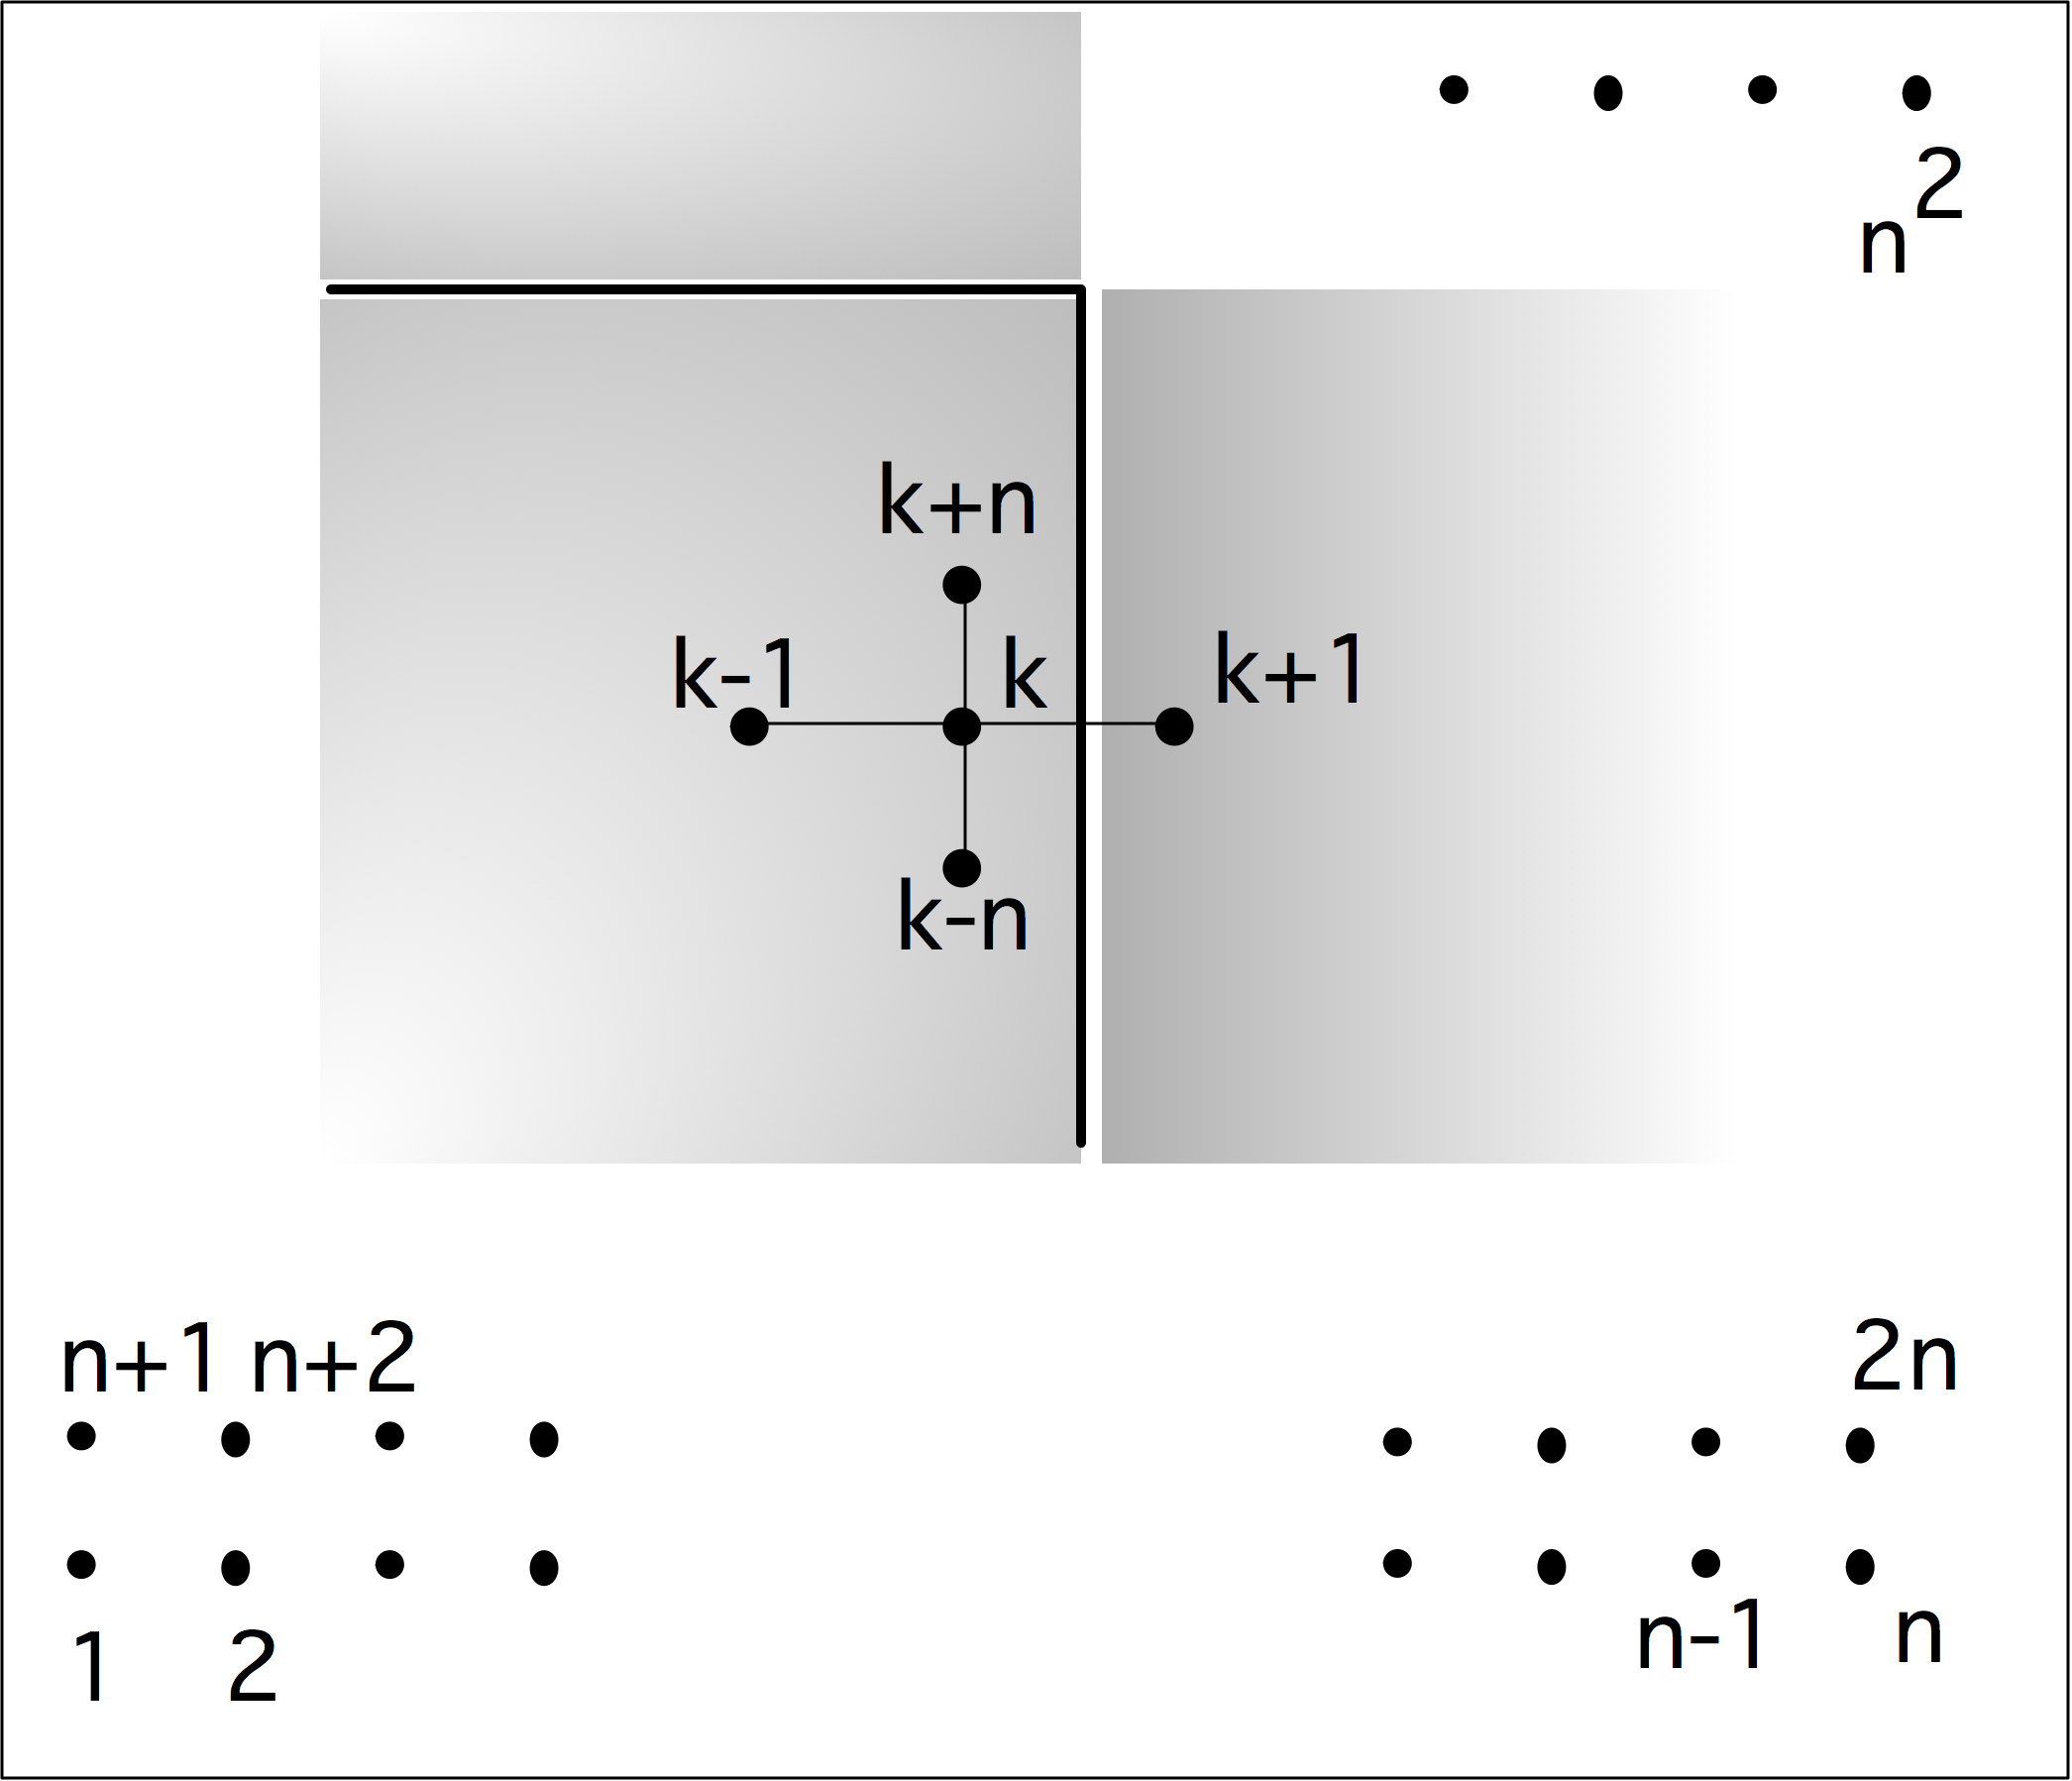
\includegraphics[scale=.12]{laplaceparallel}
  \end{quote}
  \caption{A difference stencil applied to a two-dimensional square
    domain, distributed over processors. A cross-processor connection
    is indicated..}
  \label{fig:laplaceparallel}
\end{figure}
shows how this gives rise to connections between processors: the
elements $a_{ij}$ with $i\in I_p,j\not\in I_p$ are now the `legs' of
the stencil that reach beyond a processor boundary. The set of all
such~$j$, formally defined as 
\[ G = \{ j\not\in I_p \colon 
    \exists_{i\in I_p}\colon a_{ij}\not=0 \}
\]
is known as the \indexterm{ghost region} of a processor; see
figure~\ref{fig:ghost}.
\begin{figure}
  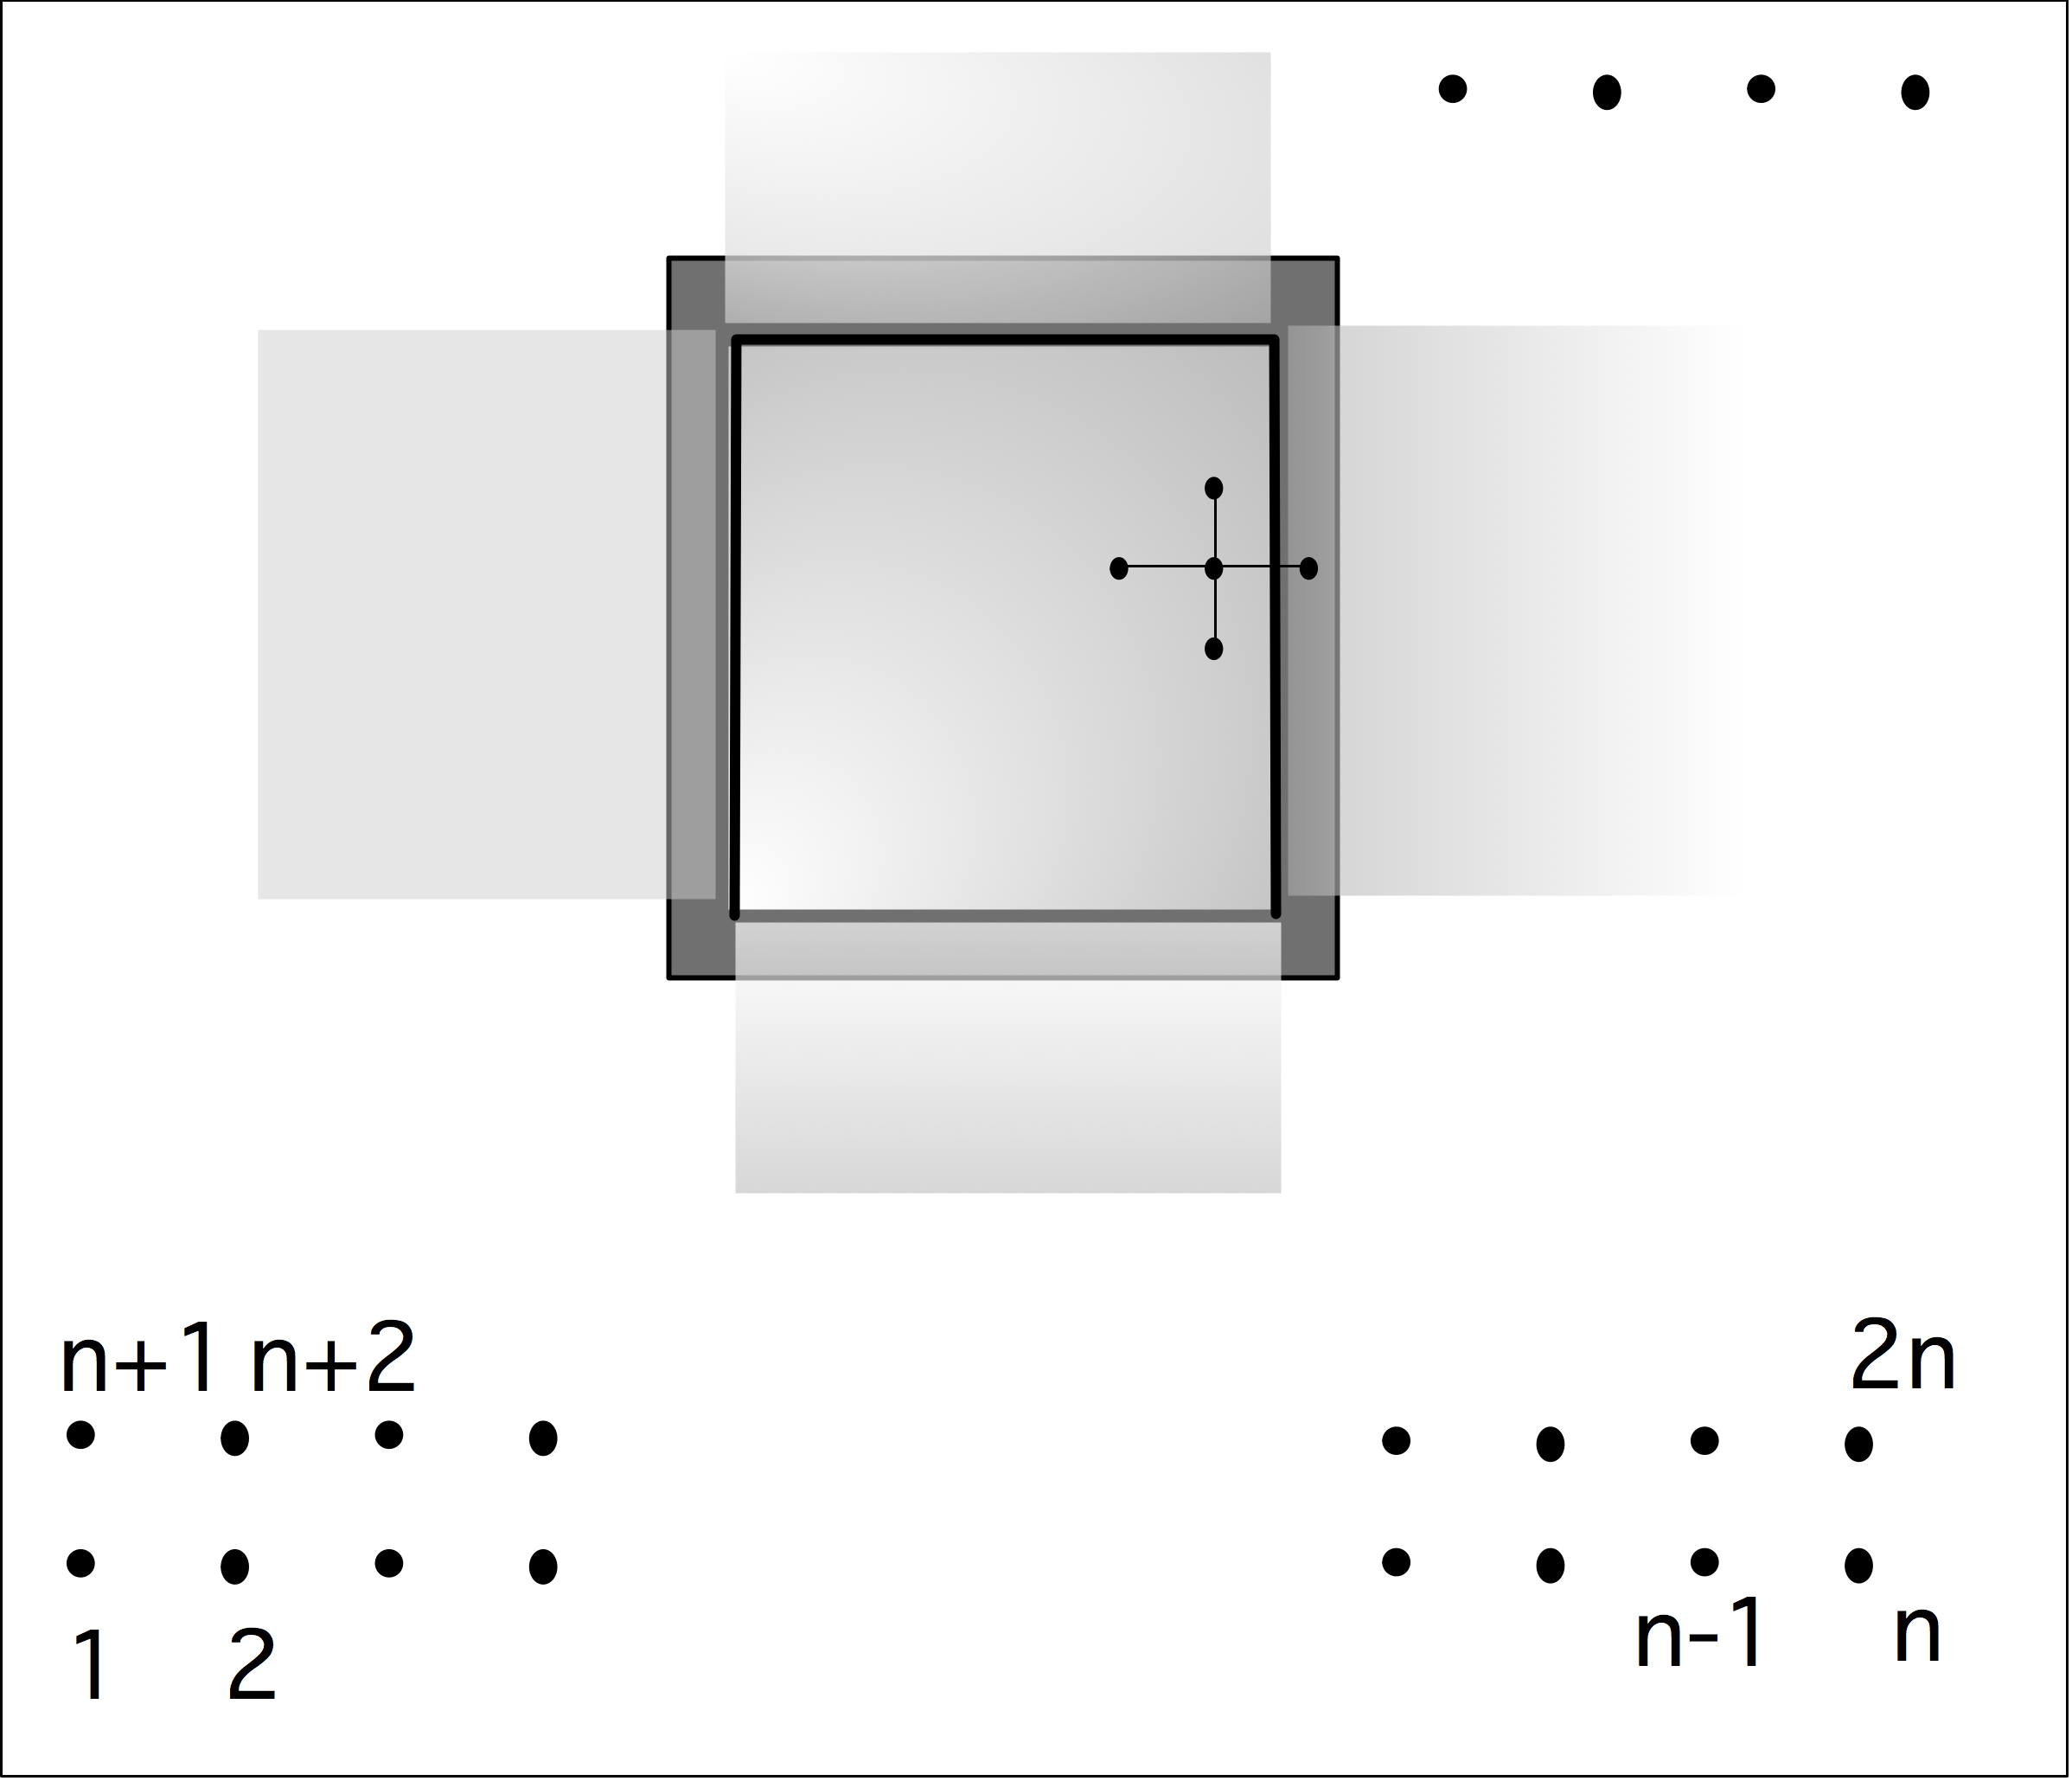
\includegraphics[scale=.12]{laplaceghost}
  \caption{The ghost region of a processor, induced by a stencil.}
  \label{fig:ghost}
\end{figure}

\begin{exercise}
  Show that a one-dimensional partitioning of the domain leads to a
  partitioning of the matrix into block rows, but a two-dimensional
  partitioning of the domain does not. You can do this in the
  abstract, or you can illustrate it: take a $4\times4$ domain (giving
  a matrix of size~16), and partition it over 4 processors. The
  one-dimensional domain partitioning corresponds to giving each
  processor one line out of the domain, while the two-dimensional
  partitioning gives each processor a $2\times2$ subdomain. Draw the
  matrices for these two cases.
\end{exercise}

\begin{figure}[ht]
  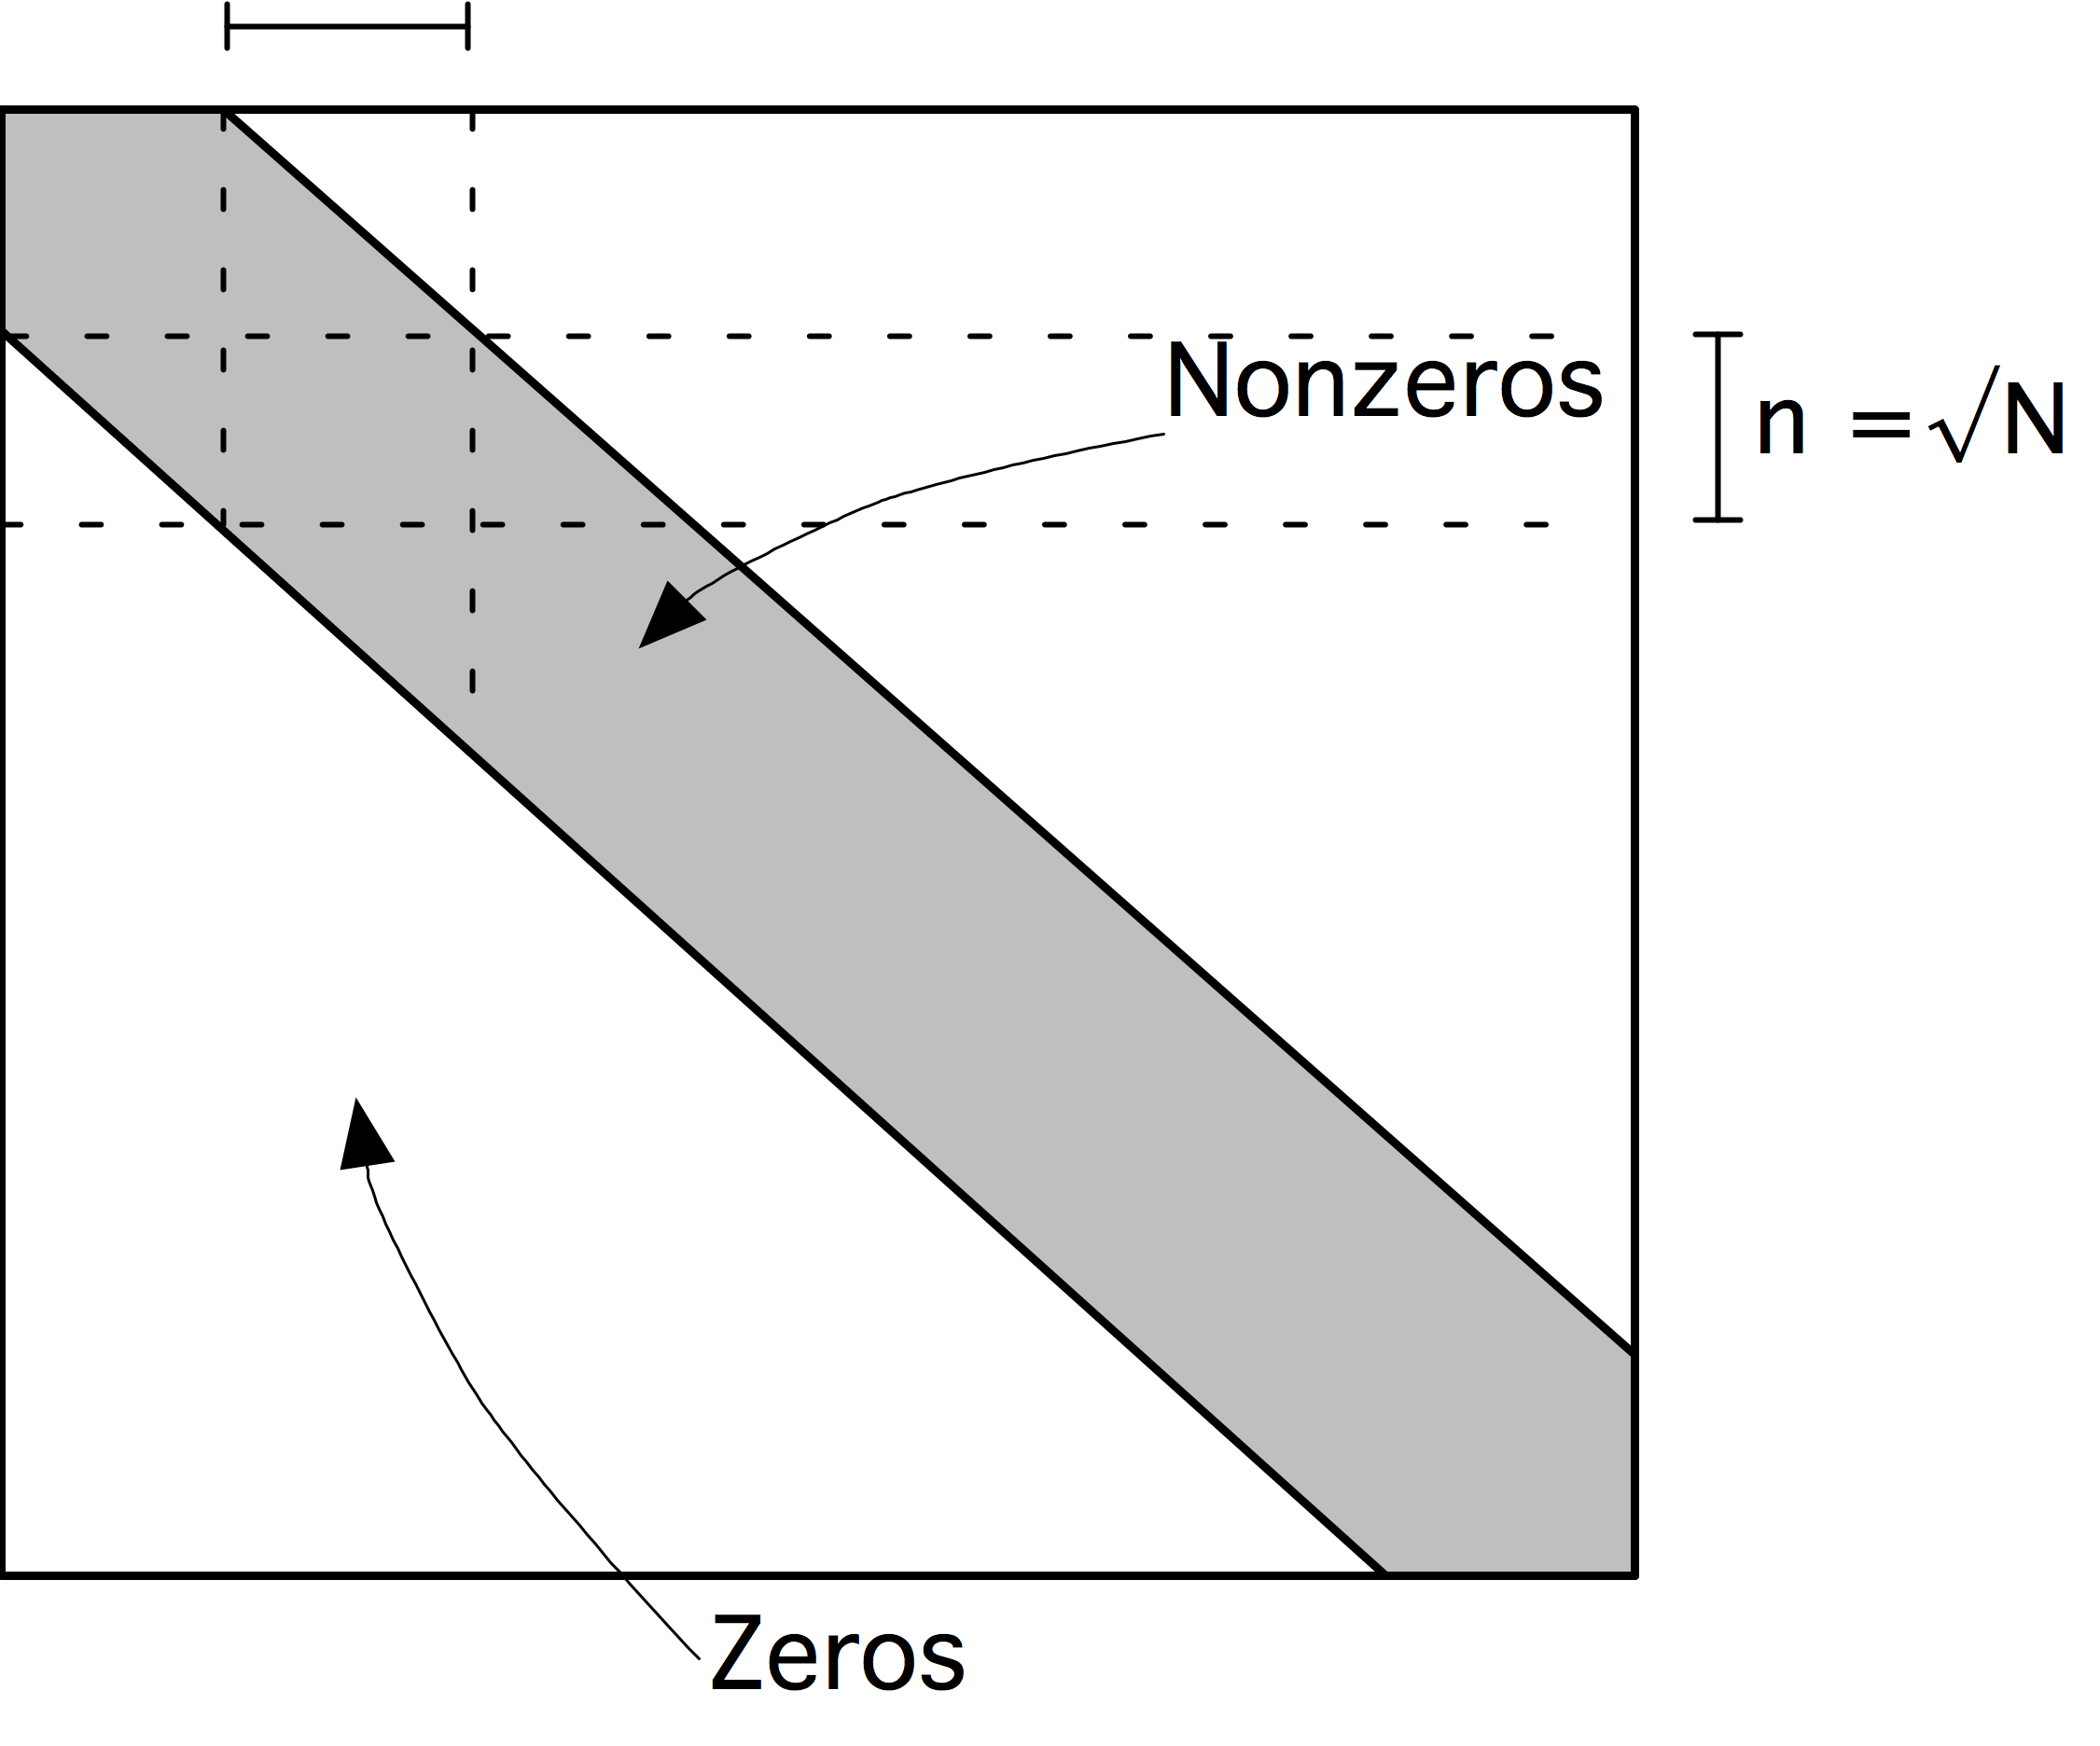
\includegraphics[scale=.1]{bandmat}
  \caption{Band matrix with halfbandwidth $\sqrt N$.}
  \label{fig:bandmat}
\end{figure}

\begin{exercise}
  \label{ex:bandmat-prod}
  Figure~\ref{fig:bandmat} depicts a sparse matrix of size~$N$ with a
  halfbandwidth~$n=\sqrt N$. That is,
  \[ |i-j|>n \Rightarrow a_{ij}=0. \]
  We make a one-dimensional distribution of this matrix over $p$
  processors, where $p=n=\sqrt N$.

  Show that the matrix-vector product using
  this scheme is weakly scalable by computing the efficiency
  as function of the number of processors
  \[ E_p = \frac{T_1}{pT_p}. \]

  Why is this scheme not really weak scaling, as it is commonly defined?
\end{exercise}

One crucial observation about the parallel sparse matrix-vector
product
is that, for each processor, the number of
other processors it is involved with is strictly limited. This has
implications for the efficiency of the operation.

In the case of the dense matrix-vector product
(section~\ref{sec:densescaling}), partitioning the matrix over the
processors by (block) rows did not lead to a scalable algorithm. Part
of the reason was the increase in the number of neighbors that each
processors needs to communicate with. Figure~\ref{fig:laplaceparallel}
shows that, for the matrix of a 5-five point stencil, this number is
limited to four.

\begin{exercise}
  Take a square domain and a partitioning of the variables of the
  processors as in figure~\ref{fig:laplaceparallel}.
  What is the maximum number of neighbors a
  processor needs to communication with for the box stencil in
  figure~\ref{fig:stencils}? In three space dimensions, what is the
  number of neighbors if a 7-point central difference stencil is
  used?
\end{exercise}

The observation that each processor communicates with just a few
neighbors stays intact if we go beyond square domains to more
complicated physical objects. If a processor receives a more or less
contiguous subdomain, the number of its neighbors will be
limited. This implies that even in complicated problems each processor
will only communicate with a small number of other processors. Compare
this to the dense case where each processor had to receive data from
\emph{every} other processor. It is obvious that the sparse case is
far more friendly to the interconnection network. (The fact that it
also more common for large systems may influence the choice of network
to install if you are about to buy a new parallel computer.)

\Level 1 {Parallel efficiency of the sparse matrix-vector product}
\label{sec:par-spmvp}

For square domains we can make the above argument formal.
Let the
unit domain $[0,1]^2$ be partitioned over $P$ processors in a $\sqrt
P\times \sqrt P$ grid. From figure~\ref{fig:laplaceparallel} we see
that every processor communicates with at most four neighbors. Let
the amount of work per processor be~$w$ and the communication time
with each neighbor~$c$. Then the time to perform the total work on a
single processor is $T_1=Pw$, and the parallel time is $T_P=w+4c$,
giving a speed up of
\[ S_P=Pw/(w+4c)=P/(1+4c/w)\approx P(1-4c/w). \]

\begin{exercise}
  Express $c$ and $w$ as functions of $N$ and~$P$, and show that the
  speedup is asymptotically optimal, under weak scaling of the problem.
\end{exercise}

\begin{exercise}
  \label{ex:scale-2d-domain}
  In this exercise you will analyze the parallel sparse matrix-vector
  product for a hypothetical, but realistic, parallel machine.
  Let the machine parameters be characterized by (see
  section~\ref{sec:latencybandwidth}):
  \begin{itemize}
  \item Network {\it Latency:} $\alpha=1\mu s=10^{-6}s$.
  \item Network {\it Bandwidth:} $1Gb/s$ corresponds to $\beta=10^{-9}$.
  \item {\it Computation rate:} A per-core flops rate of $1G$flops
    means $\gamma=10^{-9}$. This number may seem low, but note that the
    matrix-vector product has less reuse than the matrix-matrix
    product, which can achieve close to peak performance,
    and that the sparse matrix-vector product is even more
    bandwidth-bound.
  \end{itemize}
  We perform a combination of asymptotic analysis and deriving specific numbers.
  We assume a cluster of 
  $10^4$ single-core processors\footnote
  {Introducing multicore processors would complicate the story, but
    since the number of cores is $O(1)$, and the only way to grow a
    cluster is by adding more networked nodes, it does not change the
    asymptotic analysis.}. We apply this to a five-point
  stencil matrix of size $N=25\cdot 10^{10}$. This means each
  processor stores $5\cdot 8\cdot N/p=10^9$ bytes. If the matrix comes
  from a problem on a square domain, this means the domain was size
  $n\times n$ where $n=\sqrt N=5\cdot 10^5$.

  Case 1. Rather than dividing the matrix, we divide the domain, and
  we do this first by horizontal slabs of size $n\times (n/p)$. Argue
  that the communication complexity is $2(\alpha+n\beta)$ and
  computation complexity is $10\cdot n\cdot (n/p)$. Show that the
  resulting computation outweighs the communication by a factor~250.

  Case 2. We divide the domain into patches of size
  %
  $(n/\sqrt p)\times (n/\sqrt p)$.
  %
  The memory and computation time are the same as
  before. Derive the communication time and show that it is better by
  a factor of~50. 

  Argue that the first case does not weakly scale: under the
  assumption that $N/p$ is constant the efficiency will go down. 
  (Show that speedup still goes up asymptotically as~$\sqrt p$.)
  Argue that the second case does scale weakly.
\end{exercise}

The argument that a processor will only connect with a few neighbors
is based on the nature of the scientific computations. It is true for
\ac{FDM} and \ac{FEM} methods.
In the case
of the \indexac{BEM}, any subdomain needs to communicate with
everything in a radius~$r$ around it. As the number of processors goes
up, the number of neighbors per processor will also go up.

\begin{exercise}
  Give a formal analysis of the speedup and efficiency of the \ac{BEM}
  algorithm. Assume again a unit amount of work~$w$ per processor and
  a time of communication~$c$ per neighbor. Since the notion of
  neighbor is now based on physical distance, not on graph
  properties, the number of neighbors will go up. Give
  $T_1,T_p,S_p,E_p$ for this case.
\end{exercise}

There are also cases where a sparse matrix needs to be handled
similarly to a dense matrix. For instance, \indexterm{Google}'s
\indexterm{PageRank} algorithm (see section~\ref{sec:pagerank}) has at its
heart the repeated operation $x\leftarrow Ax$ where $A$~is a sparse
matrix with $A_{ij}\not=0$ if web page~$j$ links to page~$i$; see
section~\ref{sec:pagerank}. This makes $A$ a very sparse matrix, with
no obvious structure, so every processor will most likely communicate
with almost every other.


\Level 1 {Memory behavior of the sparse matrix-vector product}

In section~\ref{sec:mvp-opt} you saw an analysis of the sparse
matrix-vector product in the dense case, on a single processor. Some
of the analysis carries over immediately to the sparse case, such as
the fact that each matrix element is used only once and that the
performance is bound by the bandwidth between processor and memory.

Regarding reuse of the input and the output vector, if the matrix is
stored by rows, such as in \indexac{CRS} format (section~\ref{sec:crs}),
access to the output vector will be limited to one write per matrix
row.
On the other hand, the loop unrolling
trick for getting reuse of the input vector can not be applied
here. Code that combines two iterations is as follows:
\begin{verbatim}
for (i=0; i<M; i+=2) {
  s1 = s2 = 0;
  for (j) {
    s1 = s1 + a[i][j] * x[j];
    s2 = s2 + a[i+1][j] * x[j];
  }
  y[i] = s1; y[i+1] = s2;
}
\end{verbatim}
The problem here is that if $a_{ij}$ is nonzero, it is not guaranteed
that $a_{i+1,j}$ is nonzero. The irregularity of the sparsity pattern
makes optimizing the matrix-vector product hard. Modest improvements
are possible by identifying parts of the matrix that are small dense
blocks~\cite{ButtEijkLang:spmvp,DemEtAl:ieeeproc2004,oski}.

On a \indexac{GPU} the sparse matrix-vector product is also limited by
memory bandwidth. Programming is now harder because the \ac{GPU} has
to work in data parallel mode, with many active threads. 

An
interesting optimization becomes possible if we consider the context
in which the sparse matrix-vector product typically appears. The most
common use of this operation is in iterative solution methods for
linear systems (section~\ref{sec:iterative}), where it is applied with
the same matrix in possibly hundreds of iterations. Thus we could
consider leaving the matrix stored on the GPU and only copying the
input and output vectors for each product operation.

\Level 1 {The transpose product}
\label{sec:shared-crs-transpose}

In section~\ref{sec:crs} you saw that the code for both the regular
and the transpose matrix-vector product are limited to loop orderings
where rows of the matrix are traversed. (In section~\ref{sec:locality}
you saw a discussion of computational effects of changes in loop
order; in this case we are limited to row traversal by the storage
format.) 

In this section we will briefly look at the parallel transpose
product. Equivalently to partitioning the matrix by rows and
performing the transpose product, we look at a matrix stored and
partitioned by columns and perform the regular product.

The  algorithm for the product by columns can be given as:
\begin{quote}
    \begin{tabbing}
      $y\leftarrow 0$\\
      for \=$j$:\\
      \> for \=$i$:\\
      \>\> $y_i\leftarrow y_i+a_{ij}x_j$
    \end{tabbing}
\end{quote}
Both in shared and distributed memory we distribute outer iterations
over processors. The problem is then that each outer iteration updates
the whole output vector. This is a problem: with shared memory it
leads to multiple writes to locations in the output and in distributed
memory it requires communication that is as yet unclear.

One way to solve this would be to allocate a private output
vector~$y^{(p)}$ for each process:
\begin{quote}
    \begin{tabbing}
      $y^{(p)}\leftarrow 0$\\
      for \=$j\in$ the rows of processor $p$\\
      \> for \=all $i$:\\
      \>\> $y^{(p)}_i\leftarrow y^{(p)}_i+a_{ji}x_j$
    \end{tabbing}
\end{quote}
after which we sum $y\leftarrow\sum_py^{(p)}$.

\Level 1 {Setup of the sparse matrix-vector product}
\label{sec:par-spmvp-setup}
\index{sparse!matrix-vector product!parallel setup|(}

Above we defined sets of processes $S_p$ that contain data
to be sent to process~$p$.
It is easy enough for process $p$ to construct this set
from its part of the sparse matrix.

\begin{exercise}
  Assume that the matrix is divided over the processors by block rows;
  see figure~\ref{fig:distmvp2} for an illustration. Also assume that each processor
  knows which rows each other processor stores. (How would you implement that knowledge?)

  Sketch the algorithm by which a processor can find out who it will
  be receiving from; this algorithm should not involve any
  communication itself.
\end{exercise}

However, there is an asymmetry between sending and receiving.
While it is fairly easy for a processor to find out what other processors
it will be receiving from,
discovering who to send \emph{to} is harder.

\begin{exercise}
  Argue that this is easy in the case of a 
  \indextermsub{structurally symmetric}{matrix}:
  $a_{ij}\not=0\Leftrightarrow a_{ji}\not=0$.
\end{exercise}

In the general case, a~processor can in principle be asked to send to any other,
so the simple algorithm is as follows:
\begin{itemize}
\item Each processor makes an inventory of what non-local indices it
  needs. Under the above assumption that it knows what range of indices each
  other processor owns, it then decides which indices to get from what
  neighbors.
\item Each processor sends a list of indices to each of its
  neighbors; this list will be empty for most of the neighbors, but
  we can not omit sending it.
\item Each processor then receives these lists from all others, and
  draws up lists of which indices to send.
\end{itemize}
You will note that, even though the communication during the
matrix-vector product involves only a few neighbors for each
processor, giving a cost that is $O(1)$ in the number of processors,
the setup involves all-to-all communications, which 
have time complexity~$O(\alpha P)$

If a processor has only a few neighbors, the above algorithm is wasteful. 
Ideally, you would want space and running time proportional to the number of neighbors.
We could bring the receive time in the setup if we knew how many messages
were to be expected. That number can be found:
\begin{itemize}
\item Each processor makes an array \n{need} of length~$P$, where \n{need[i]}
  is~1 if the processor needs any data from processor~$i$, and zero otherwise.
\item A \indexterm{reduce-scatter} collective on this array, with a
  sum operator, then leaves on each processor a number indicating how
  many processors need data from it.
\item The processor can execute that many receive calls.
\end{itemize}
The reduce-scatter call has time complexity $\alpha\log P+\beta P$,
which is of the same order as the previous algorithm, but 
probably with a lower proportionality constant.

The time and space needed for the setup can be reduced to $O(\log P)$ with some
sophisticated trickery~\cite{Falgout:scalable-hypre,Hoefler:2010:SCP}.

\index{sparse!matrix-vector product!parallel setup|)}

% LocalWords:  Eijkhout sparsity discretized subdomain halfbandwidth
% LocalWords:  multicore FDM FEM BEM PageRank CRS GPU PDE blockrows
% LocalWords:  nonzeros
